\section{Test: Linear model}
The purpose of this chapter is to show and discuss the performance results of the LQI controller derived in \cref{sec:ctrl-design} on the linear model derived in \cref{sec:linear_model}. The controller is benchmarked against the original FLC controller with regards to both rotor speed control and fore-aft movement dampening capability. Prior to the test the LQI controller has been tuned such that a satisfactory performance was achieved on the linear model. 

It is expected that the LQI controller will perform much better in damping the fore-aft movement than the original FLC PI controller. It is also expected to perform better in generator speed control despite the fact that the original FLC controller has been thoroughly tuned to achieve the best possible generator speed tracking performance. The reason for this hypothesis is less obvious. The reason is that the LQI controller has been tuned on the simple linear model and not in VTS like the FLC PI controller. Thus potential unforeseen consequences of having an aggressive controller in a more realistic environment are not discovered until it is tested in VTS.

Test results are shown for both frequency and time domain.


\subsection{Test framework}
Matlab is used to make bode plots and Matlab Simulink is used to run time simulations. The Matlab \textit{connect()} function is utilized with component models defined on a specific form to gain transfer functions or state space systems from one or more inputs to one or more outputs. From these the \textit{bode()} Matlab function is used to make bode plots. 

Time simulations are made with the FLC PI and LQI controlled linear models from the $ A $, $ B $ and $ C $ system matrices controller gains $ K $. In \cref{fig:simulink_setup2} the Simulink simulation setup is seen. Two systems are observed with the top one containing the original FLC PI controller without FATD enabled and the bottom one being the one with the designed LQI controller. While not directly apparent because of the missing state feedback, the top system is a closed loop system with the controller gain $ K $ contained in the $ A $ and $ B $ matrix. The reason for this is simply that the FLC component described in \cref{sec:comp_flc} is defined as a generic component model and conveniently combined with the Matlab \textit{connect()} function to yield a full closed-loop system. 

From the left the free wind disturbance deviation from the operating point is observed entering both systems. The simulation is run for a total of 1000 seconds.
% and at time $ T = 300 $ a step of 2 m/s is made on $ v_{free} $. 
The simulations are initialized at the operating point except for the tower top position $ p_y $ which is initialized with a deviation of 5 m to provoke a response from both systems.
\begin{figure}[ht]
	\centering
	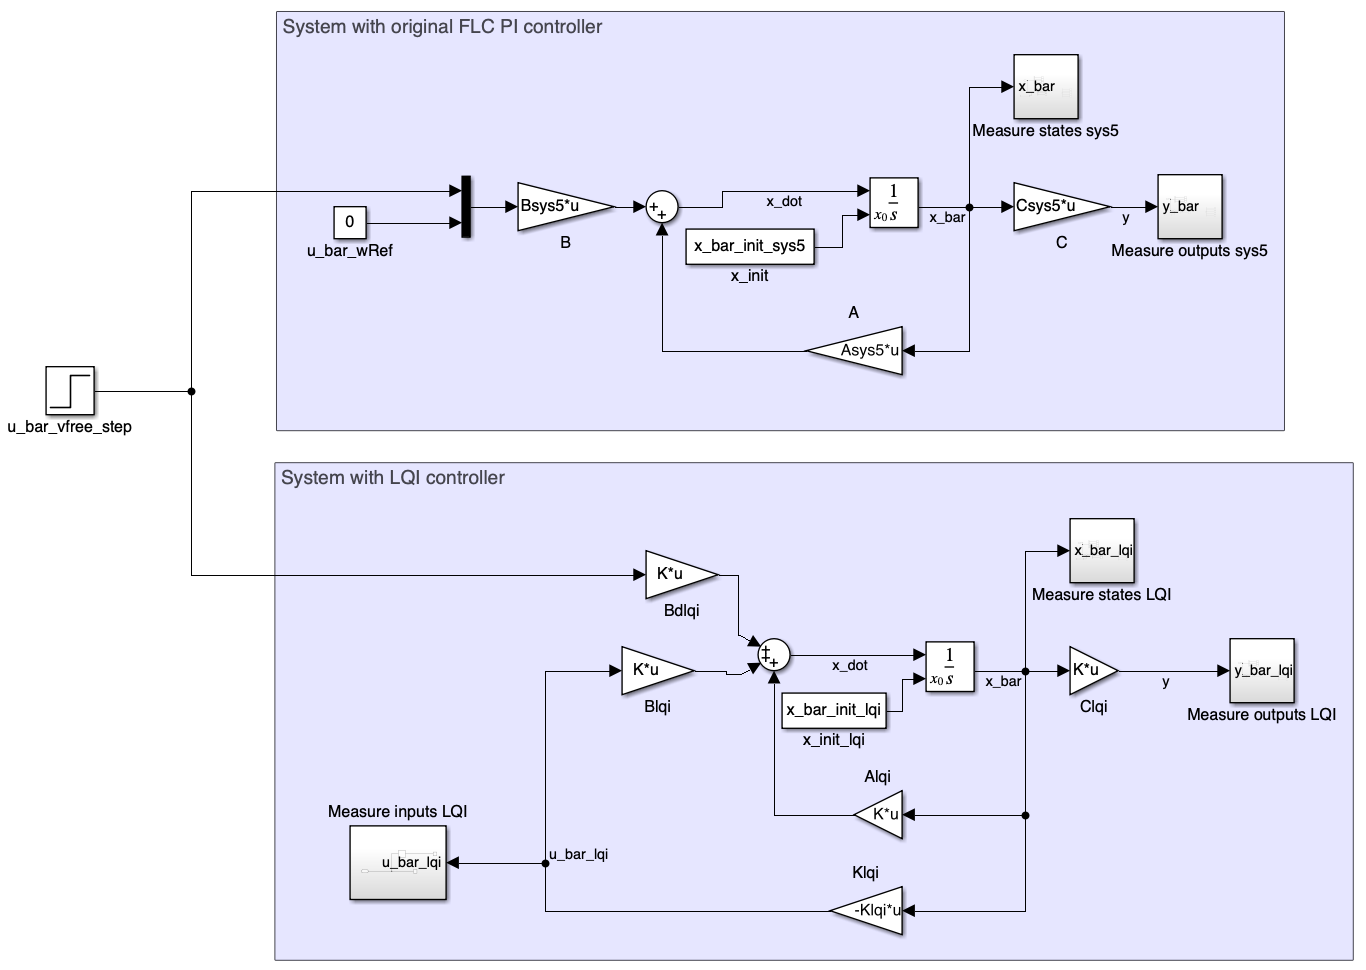
\includegraphics[width=0.95\linewidth]{Graphics/TestResults/linearModPerf/simulink_setup.png}
	\caption{The Matlab Simulink setup. The step in the free wind speed is observed entering the system from the left through the }
	\label{fig:simulink_setup2}
\end{figure}


\subsection{Test results}
In this section the test results are both presented and discussed.


\subsubsection{Frequency Domain}
In figure \cref{fig:script_vfreeTovy} the frequency response from the free wind disturbance $ v_{free} $ to the surge direction tower top velocity $ v_y $ is seen. Both the FLC PI system and LQI system are plotted for easy comparison. The plotted frequency range is between 0.01 and 0.3 Hz because this is the frequency range of interest. In figure \cref{fig:script_vfreeToW} the frequency response $ v_{free} $ to the rotor speed $ \Omega $ is seen. The LQI controller is observed yielding much greater dampening of the eigenfrequency for both plots. The gain from $ v_{free} $ to $ \Omega $ is around 10 to 13 dB higher until around 0.05 Hz. \todo[inline]{Ret disse tal når controller er tunet.}

\begin{figure}[ht]
	\centering
	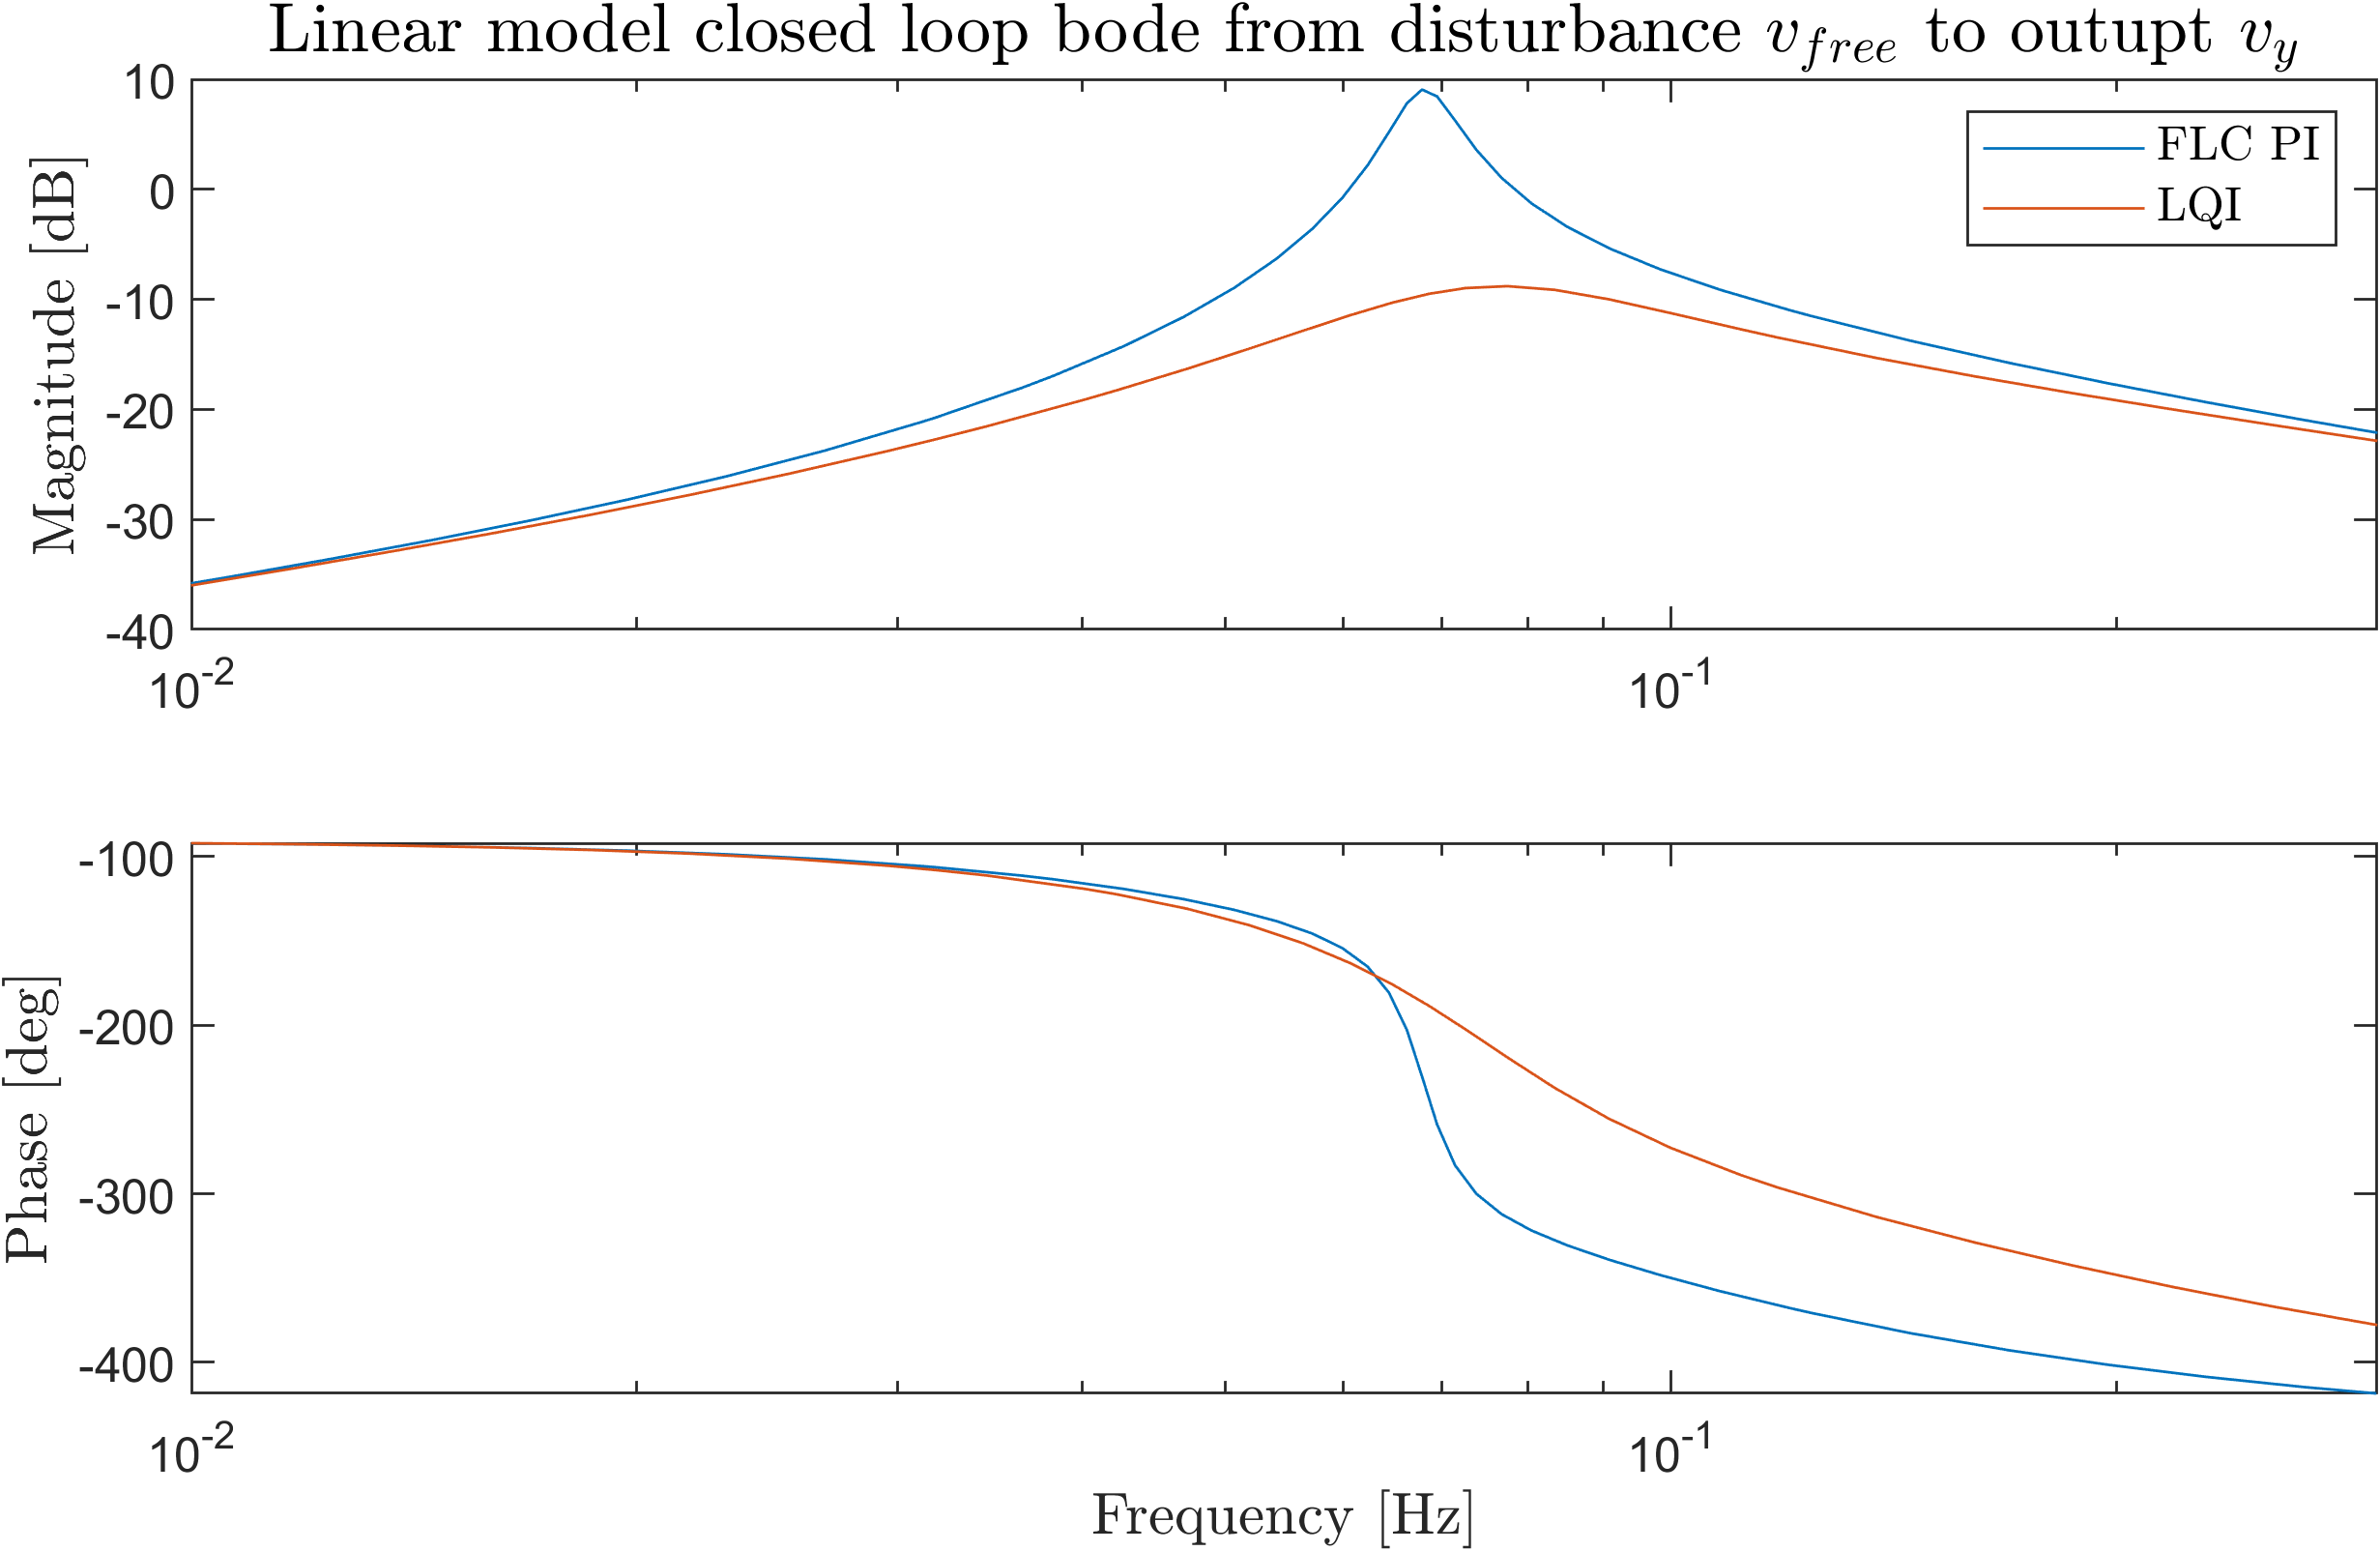
\includegraphics[width=0.7\linewidth]{Graphics/TestResults/linearModPerf/script_vfreeTovy.png}
	\caption{Frequency response from the free wind as observed by the rotor ($ v_{free} $) to the rotor speed  ($ \Omega $) of the linear model with comparison between the original FLC PI controller and the developed LQI controller.}
	\label{fig:script_vfreeTovy}
\end{figure}

\begin{figure}[ht]
	\centering
	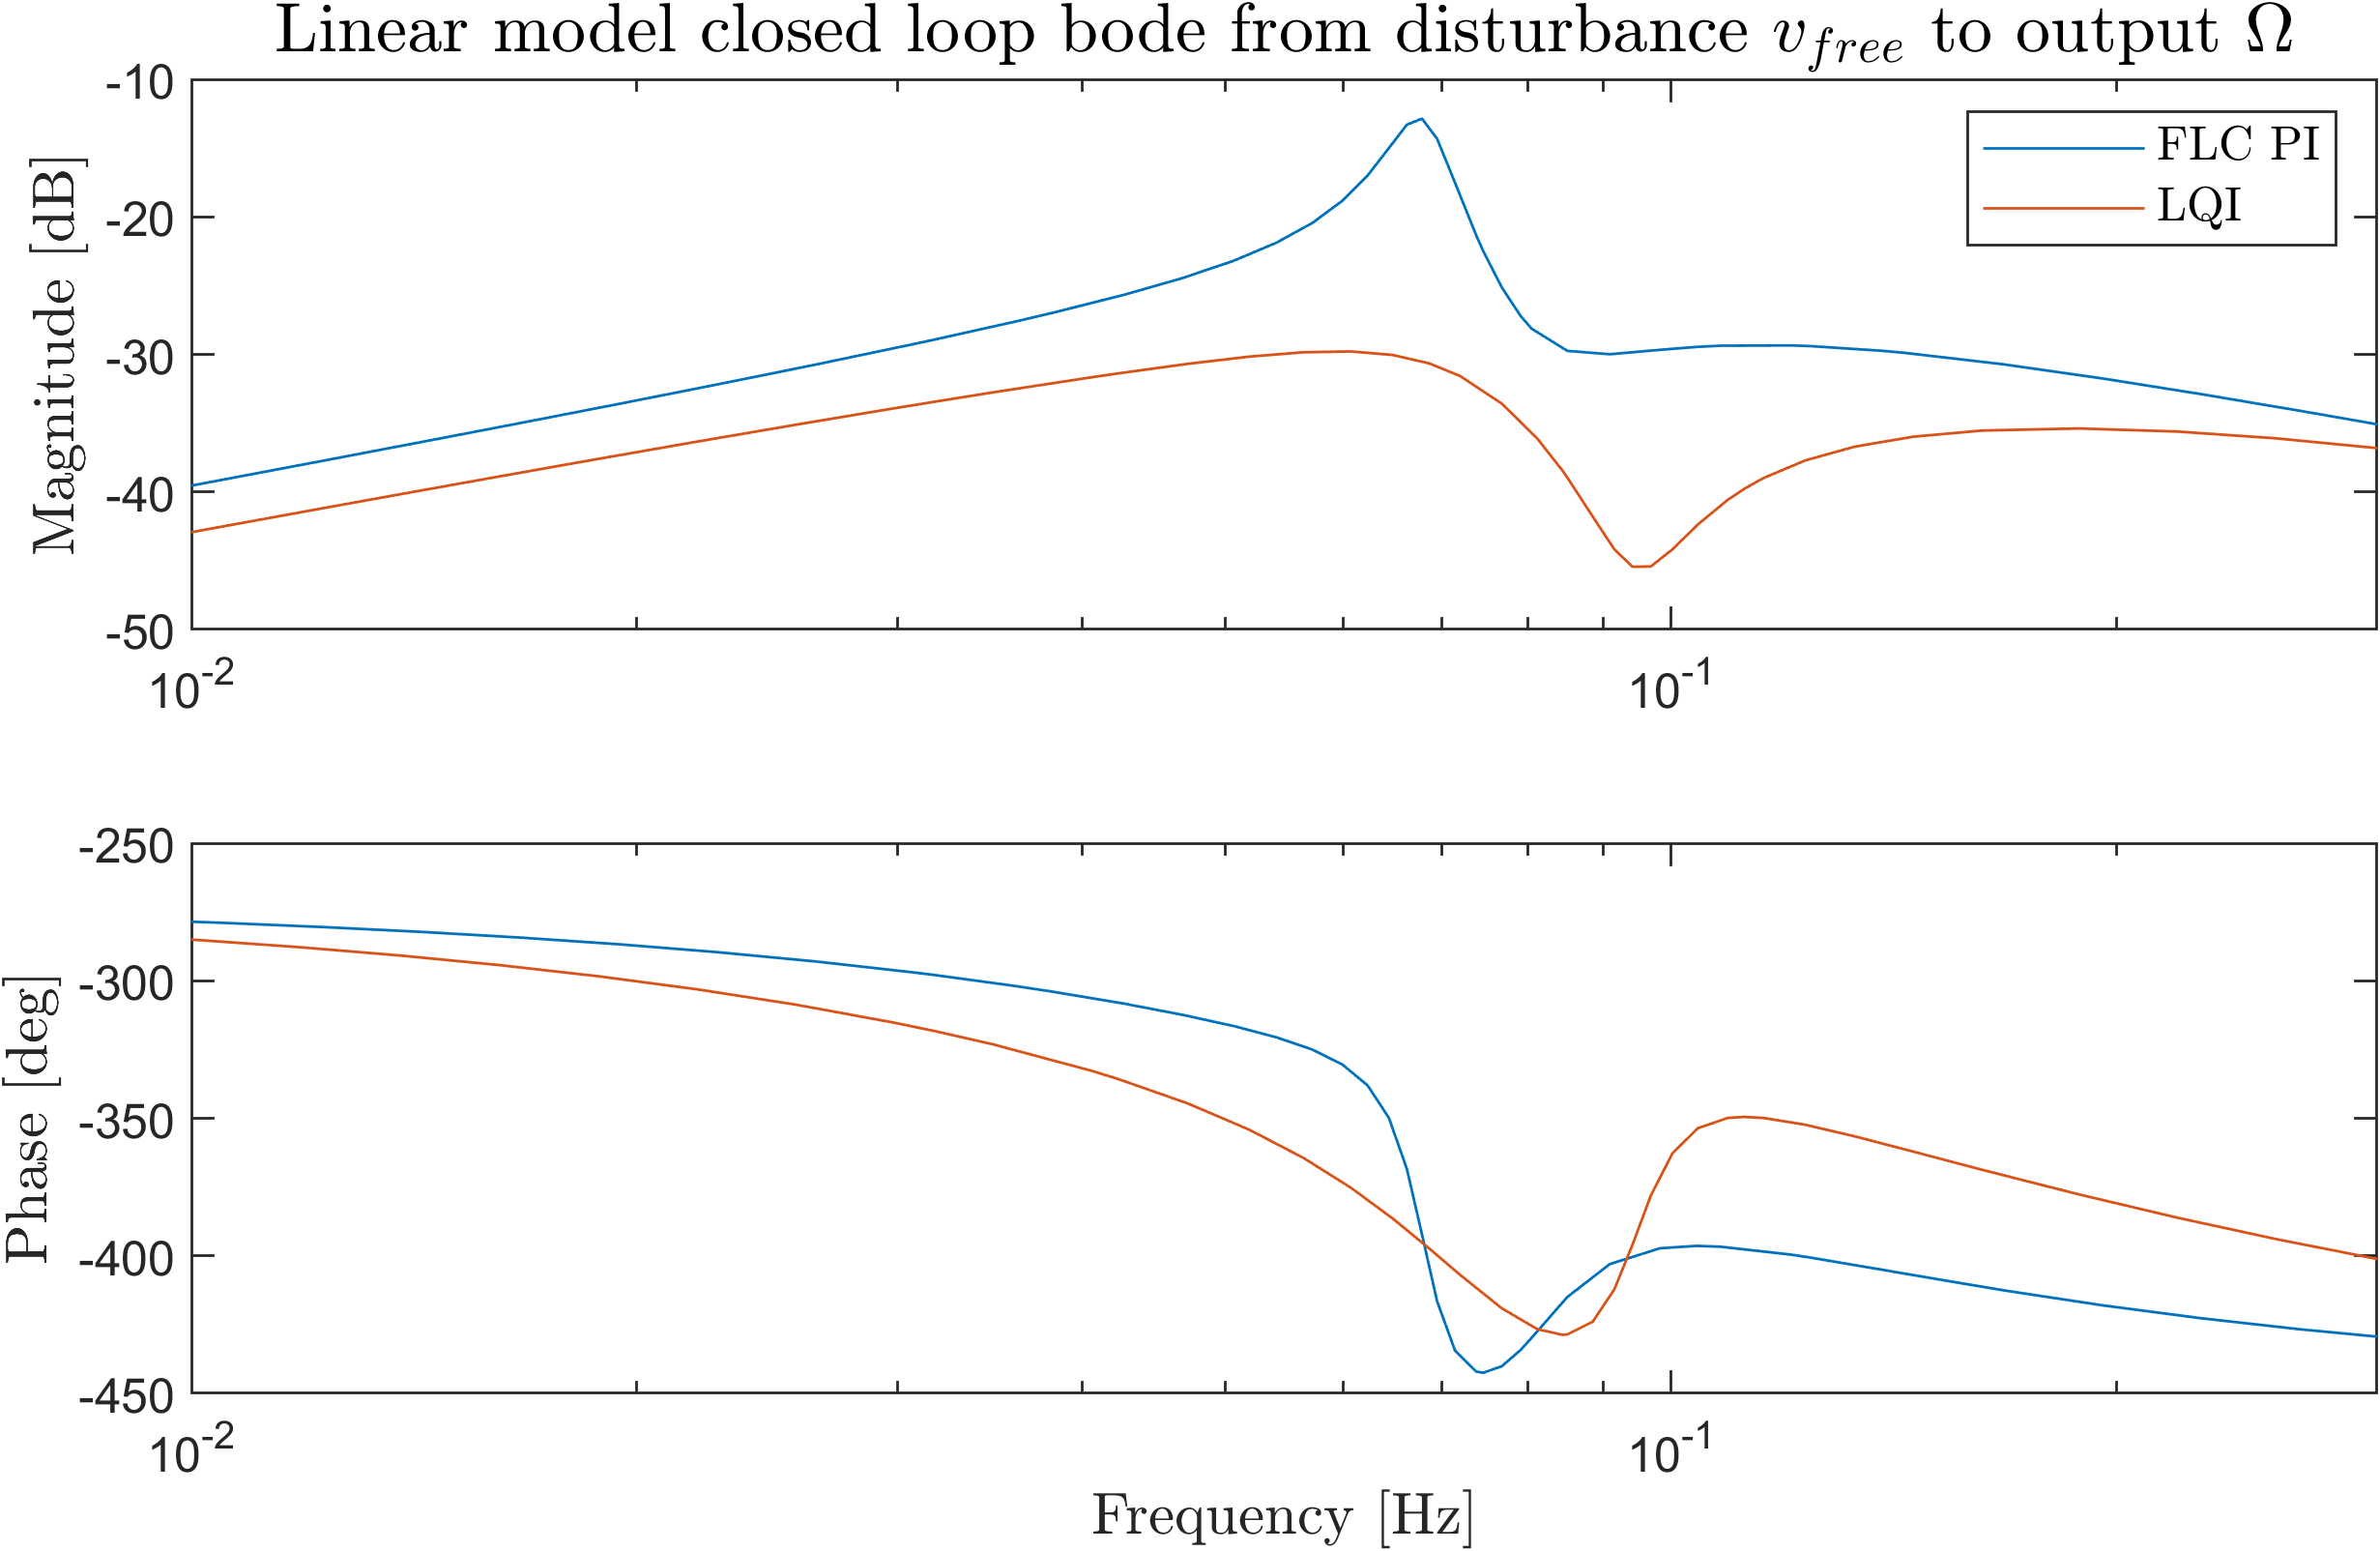
\includegraphics[width=0.7\linewidth]{Graphics/TestResults/linearModPerf/script_vfreeToW.png}
	\caption{Frequency response from the free wind as observed by the rotor ($ v_{free} $) to the surge direction tower top velocity ($ v_y $) of the linear model with comparison between the original FLC PI controller and the developed LQI controller.}
	\label{fig:script_vfreeToW}
\end{figure}

\clearpage
\subsubsection{Time domain}
In \cref{fig:02_W_py_vy_comp} the rotor speed, surge direction position and surge direction velocity is plotted in time from 0 to 1000 seconds. Both the FLC PI and LQI controlled systems are plotted for easy comparison. \cref{fig:03_W_py_vy_comp_zoom} shows a plot zoomed in at the disturbance step at 300 seconds.
%\begin{figure}[ht]
%	\centering
%	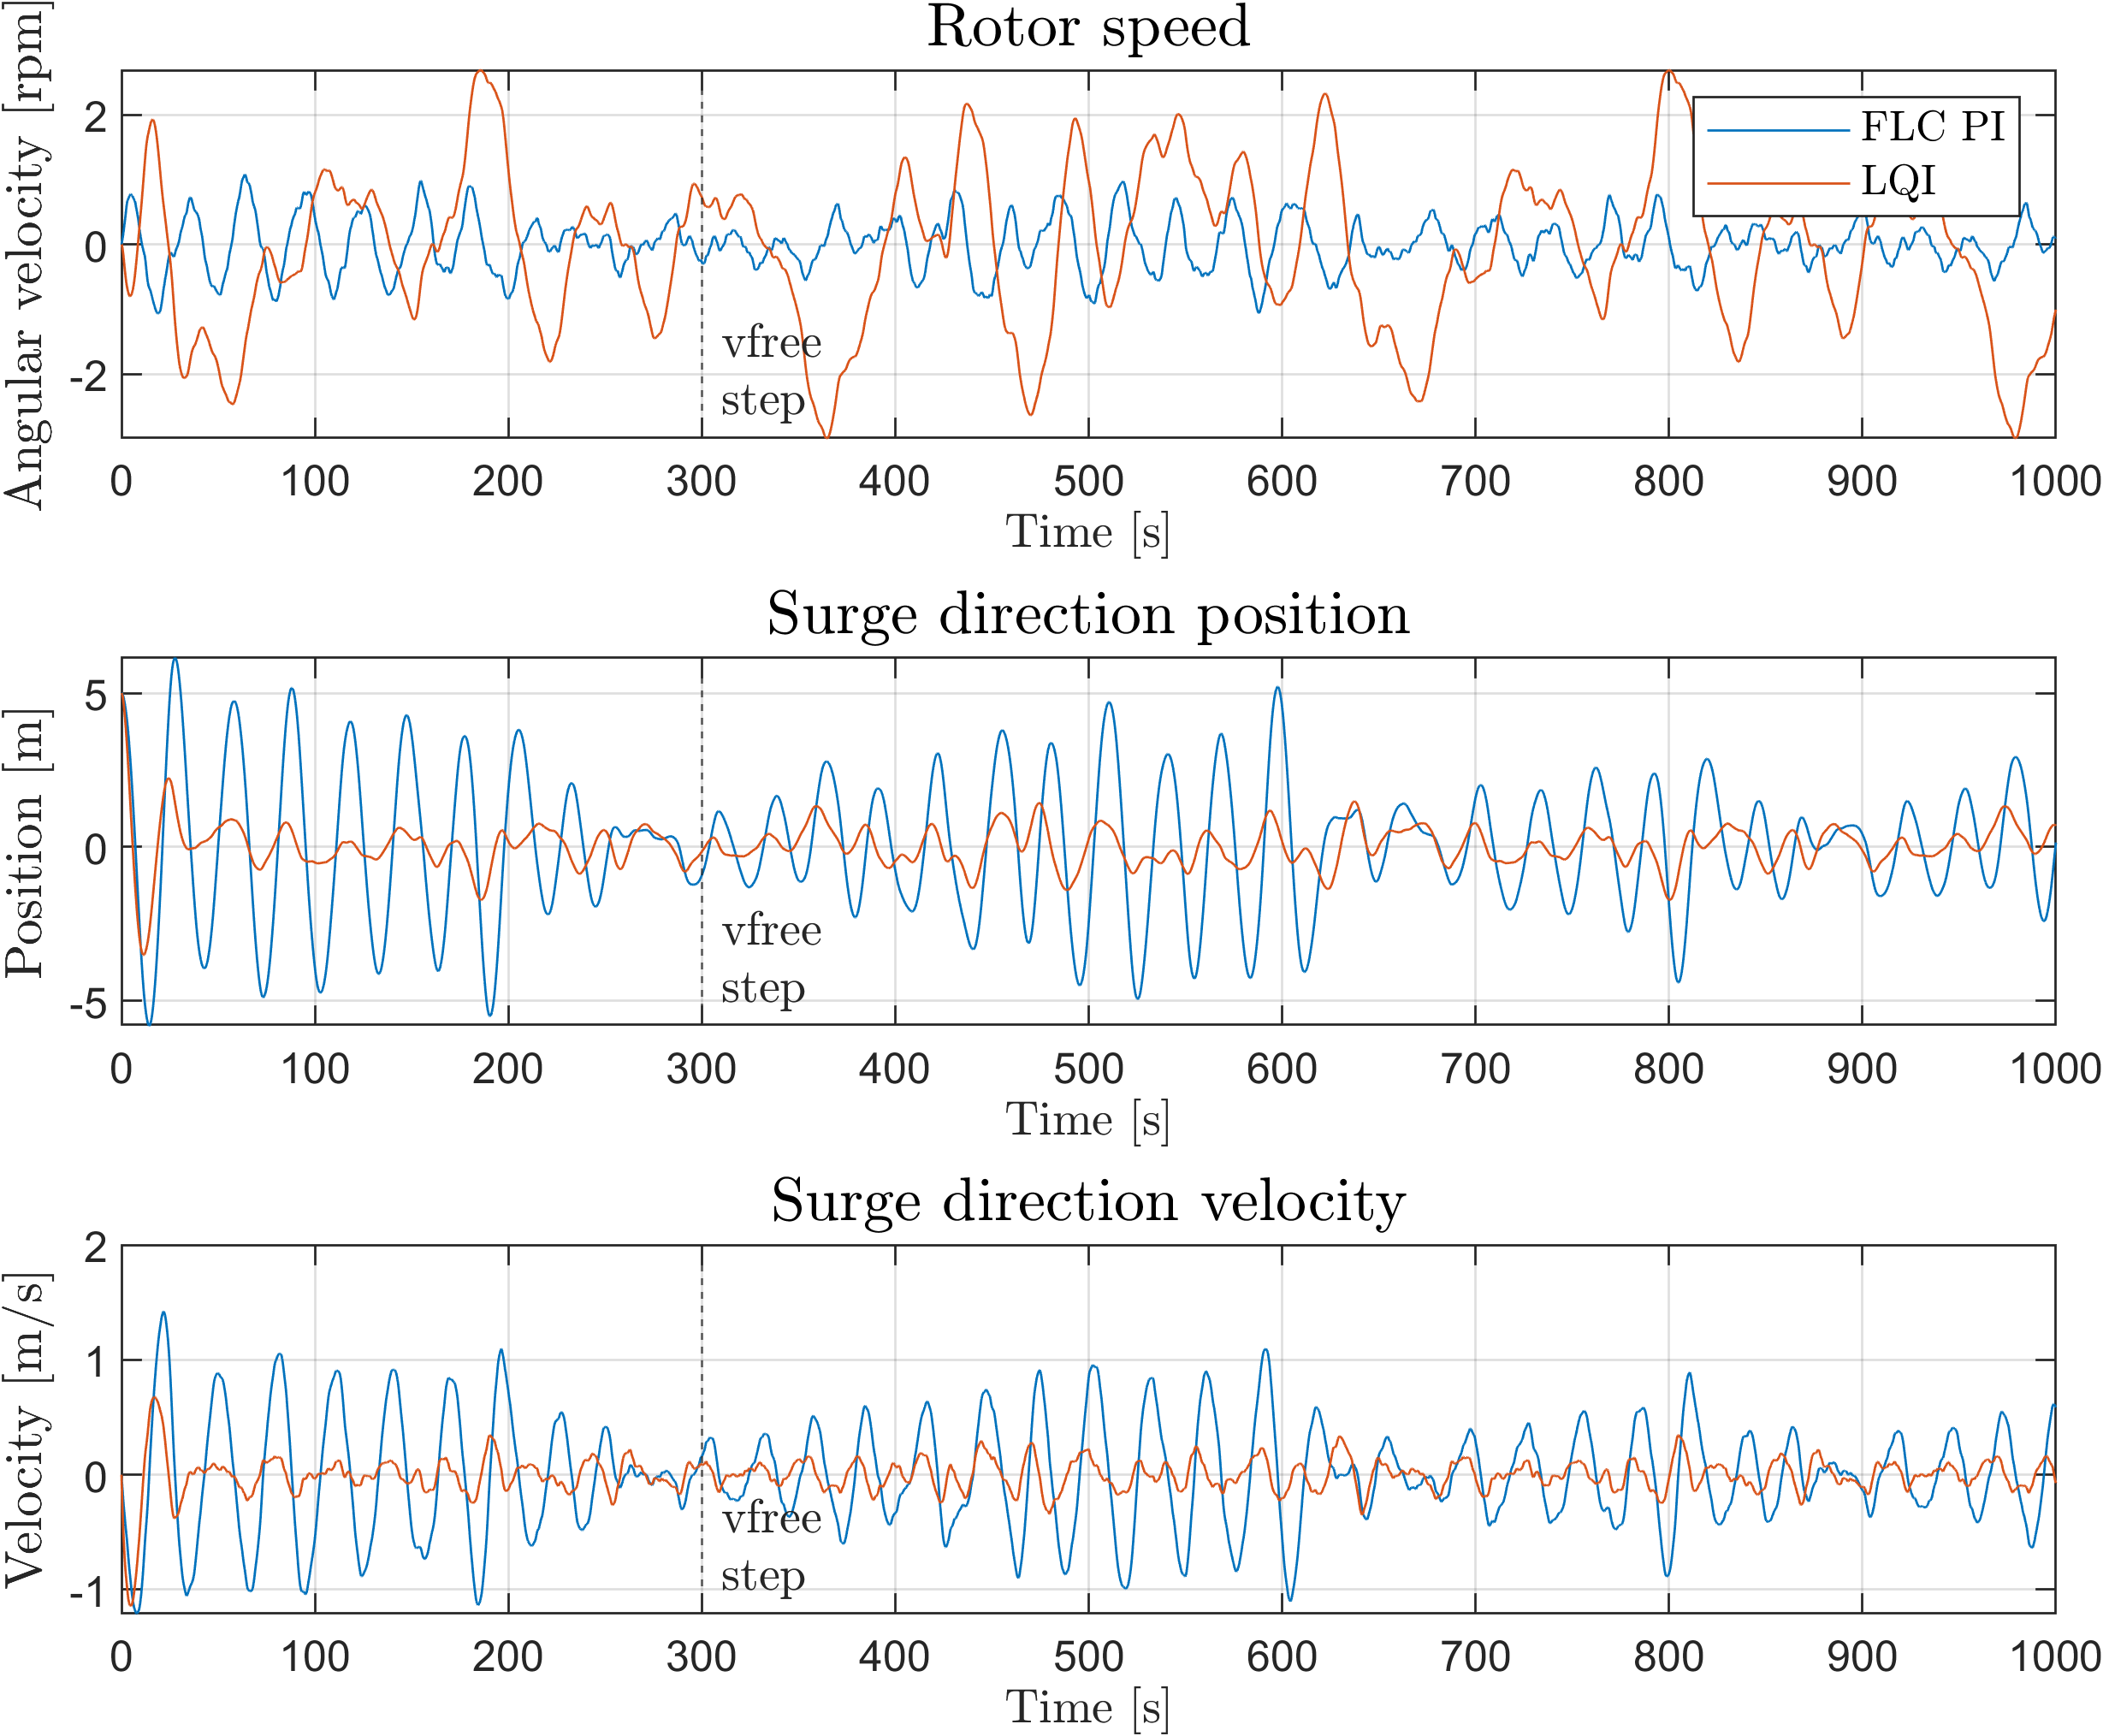
\includegraphics[width=0.7\linewidth]{Graphics/TestResults/linearModPerf/sim_02_W_py_vy_comp.png}
%	\caption{Simulink simulation results. The 10 m deviation initialization of the tower top position is visible from the \textit{Surge direction position} at 0 s.}
%	\label{fig:sim_02_W_py_vy_comp}
%\end{figure}
%
%\begin{figure}[ht]
%	\centering
%	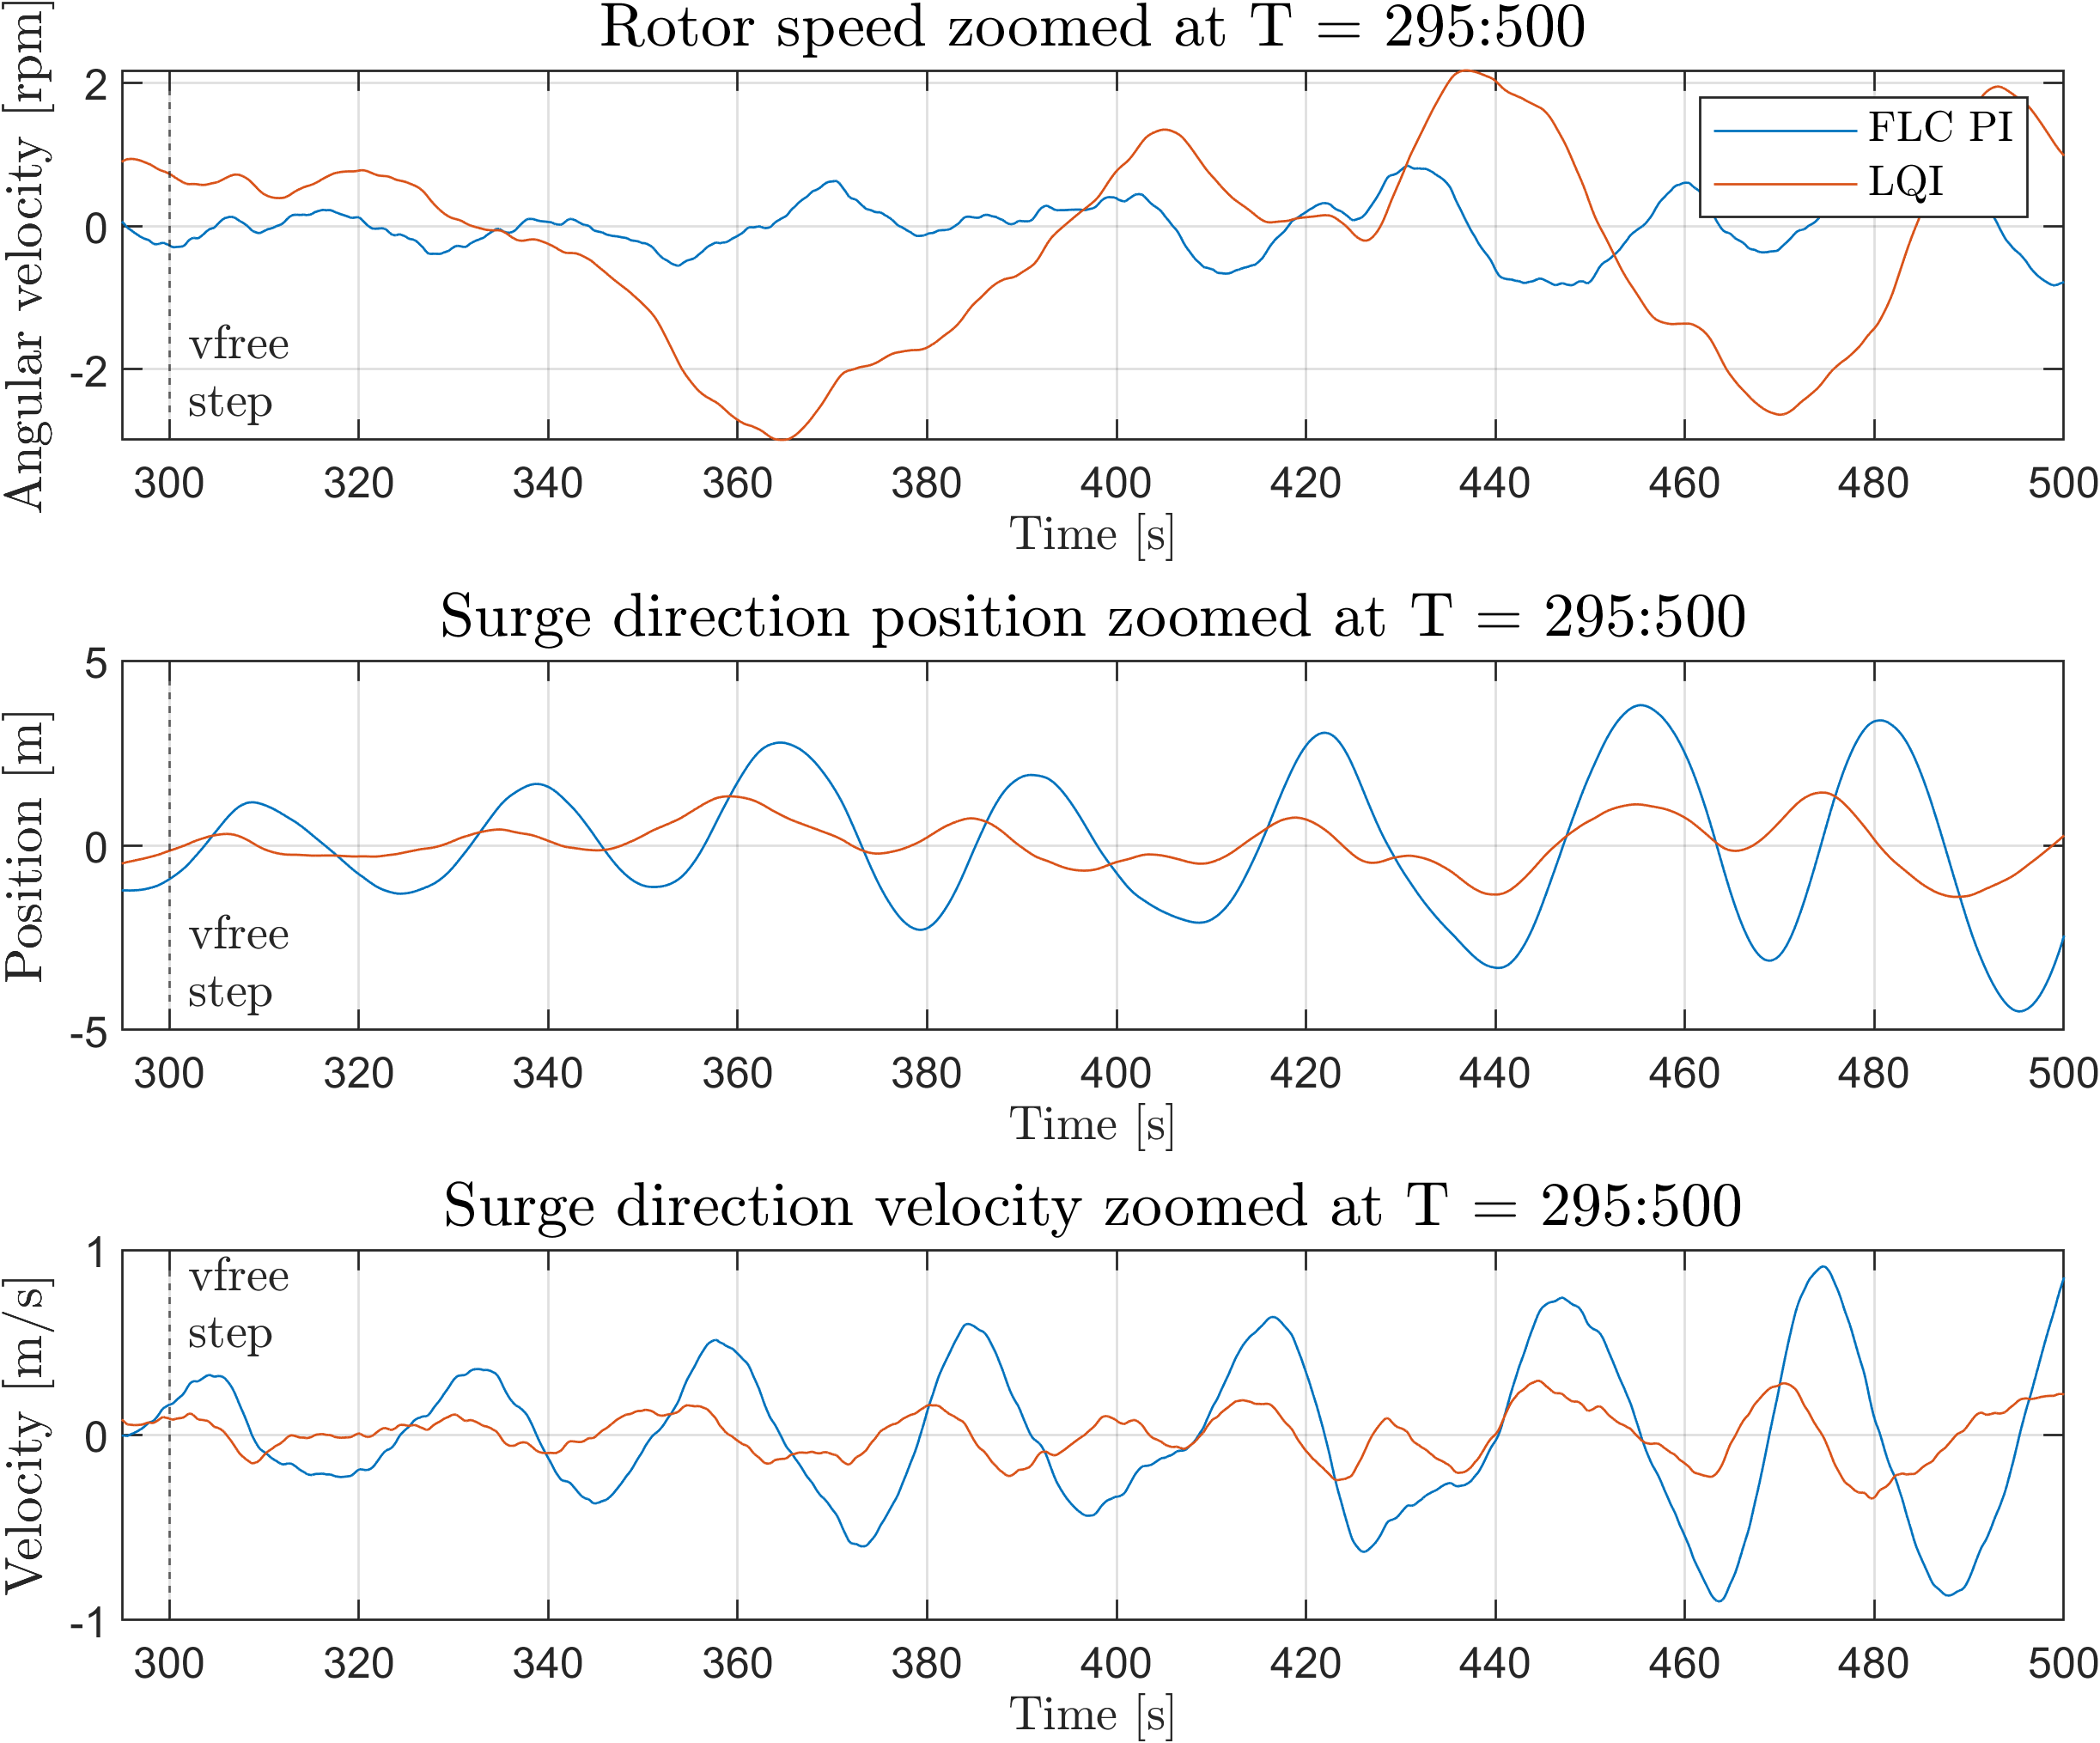
\includegraphics[width=0.7\linewidth]{Graphics/TestResults/linearModPerf/sim_03_W_py_vy_comp_zoom.png}
%	\caption{Simulink simulation results. Zoom at the disturbance step.}
%	\label{fig:sim_03_W_py_vy_comp_zoom}
%\end{figure}
%
%\begin{figure}[ht]
%	\centering
%	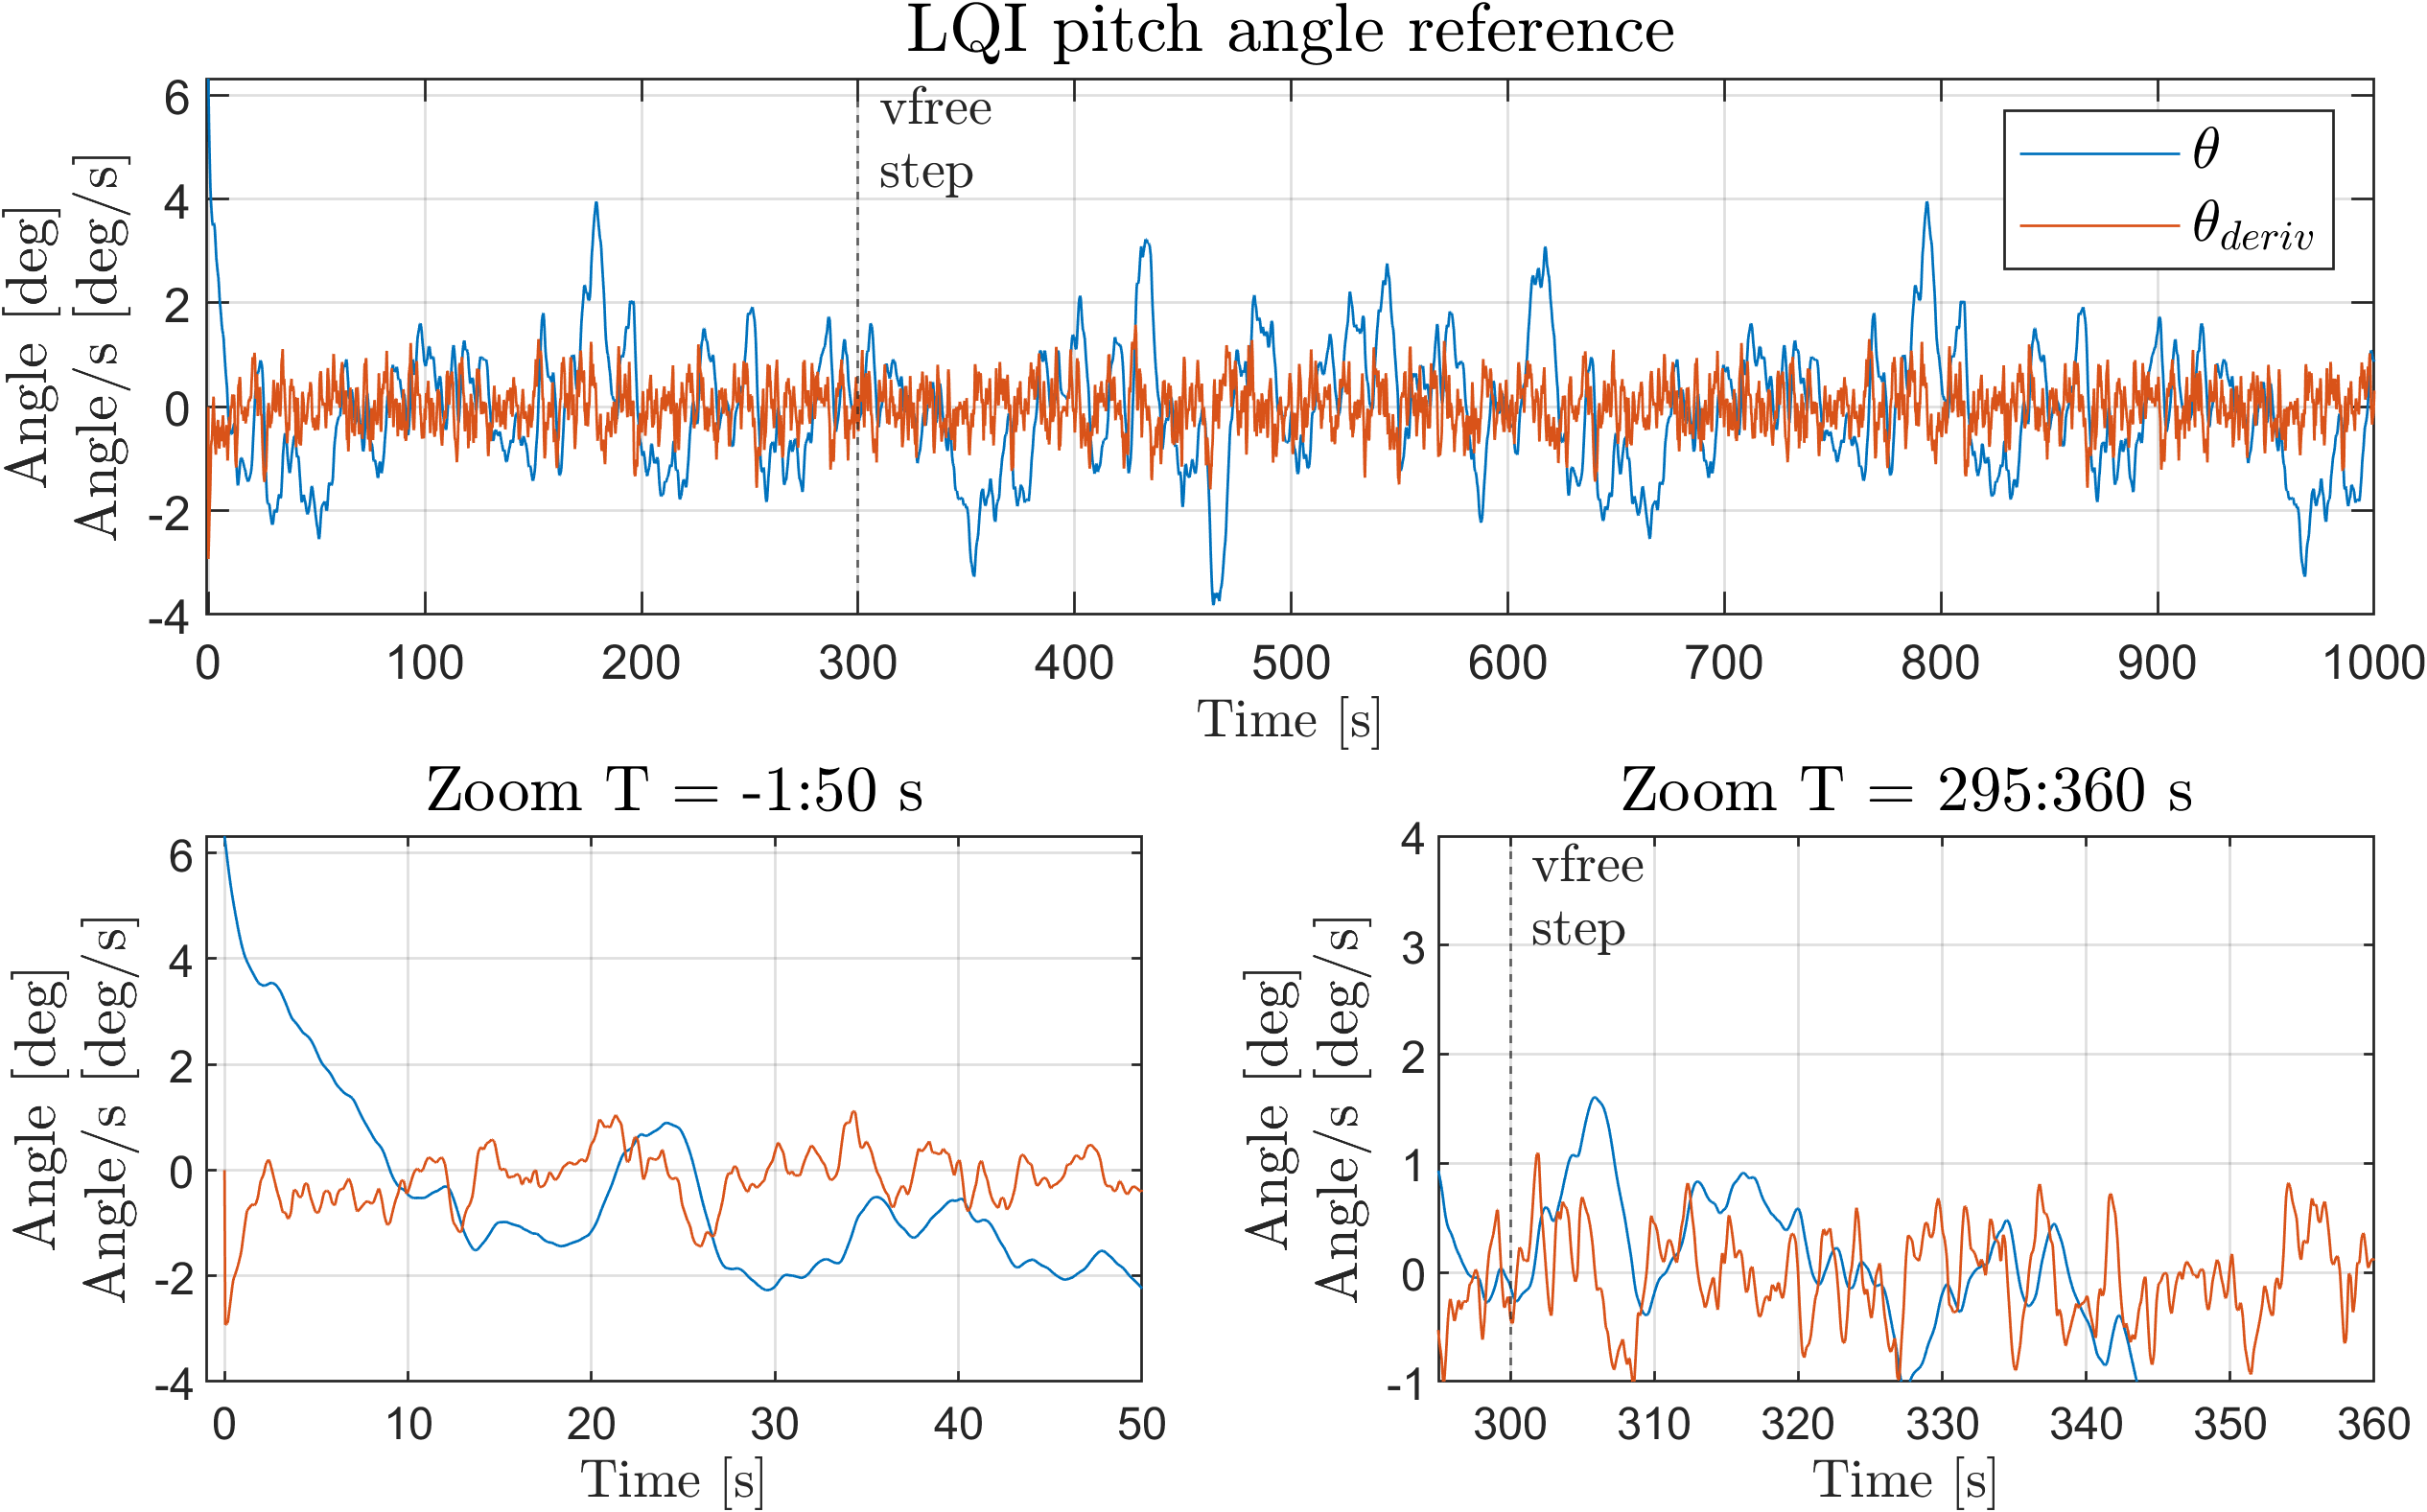
\includegraphics[width=0.7\linewidth]{Graphics/TestResults/linearModPerf/sim_01_pitch.png}
%	\caption{Simulink simulation results. Bottom left and right plots are zommed in at 0 to 50 s and 295 to 360 s.}
%	\label{fig:sim_01_pitch}
%\end{figure}

\begin{figure}[ht]
	\centering
	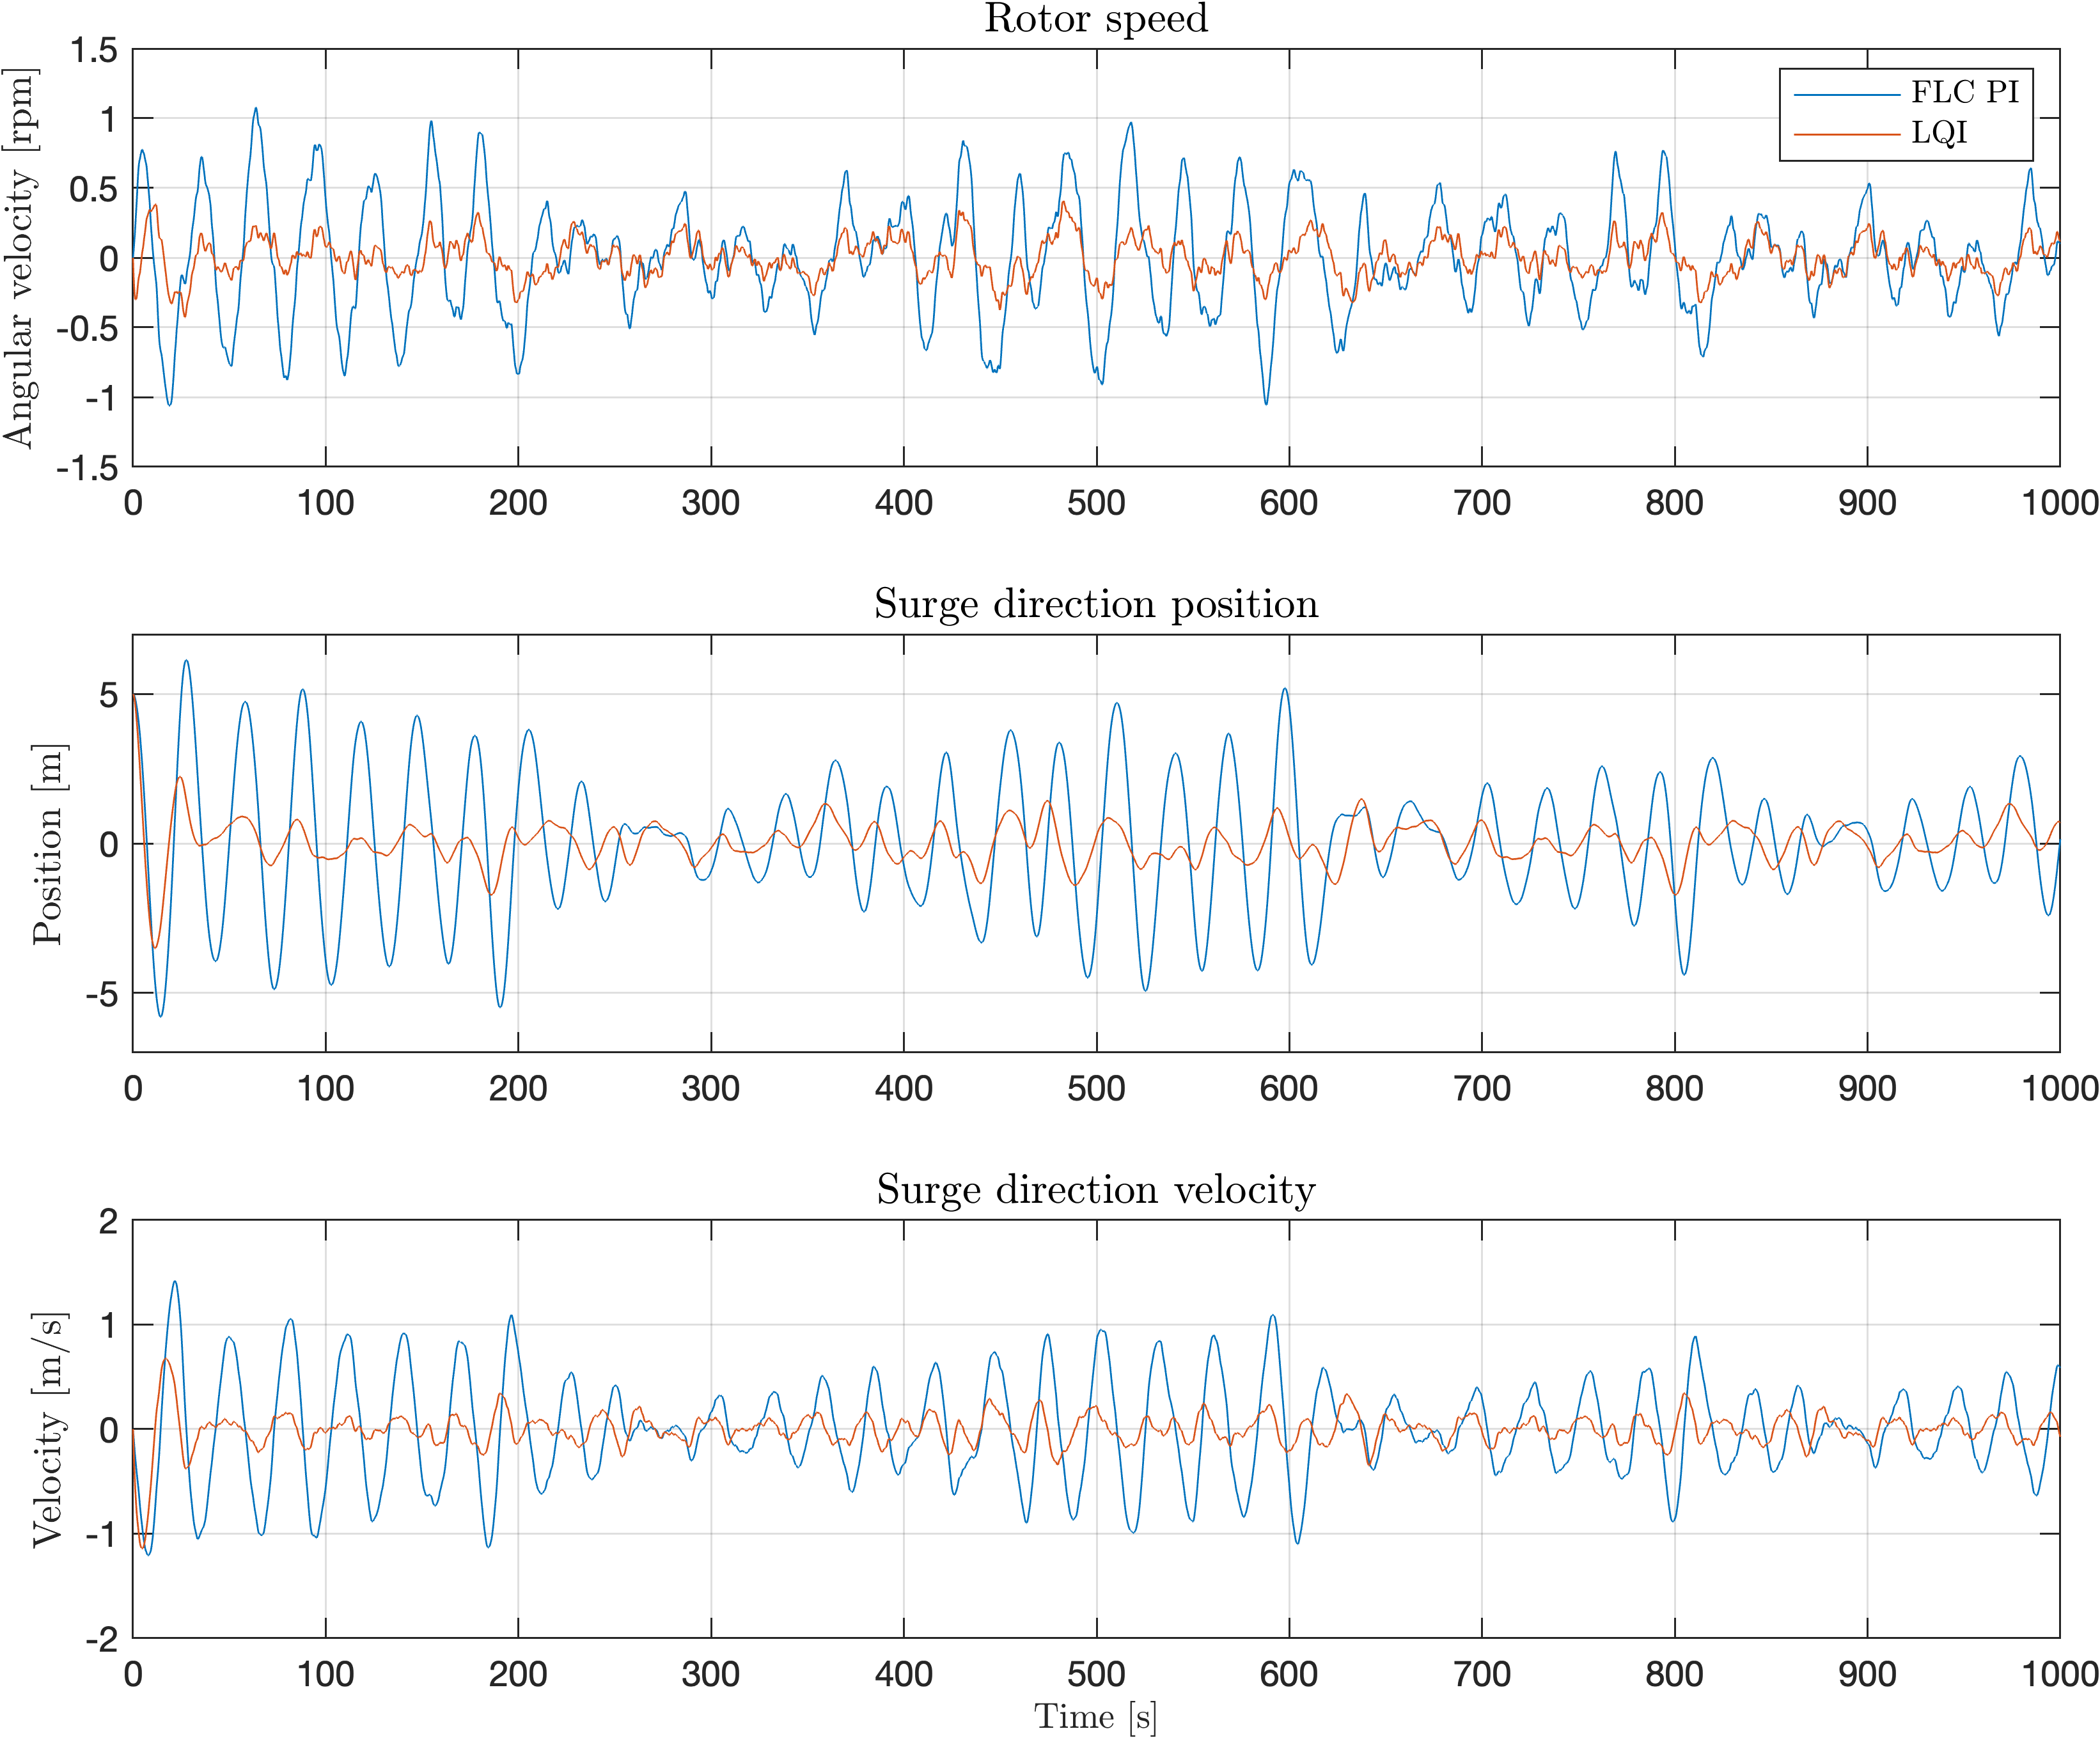
\includegraphics[width=0.7\linewidth]{Graphics/TestResults/linearModPerf/sim_11_W_py_vy_comp.png}
	\caption{Simulink simulation results. The 10 m deviation initialization of the tower top position is visible from the \textit{Surge direction position} at 0 s.}
	\label{fig:sim_02_W_py_vy_comp}
\end{figure}

\begin{figure}[ht]
	\centering
	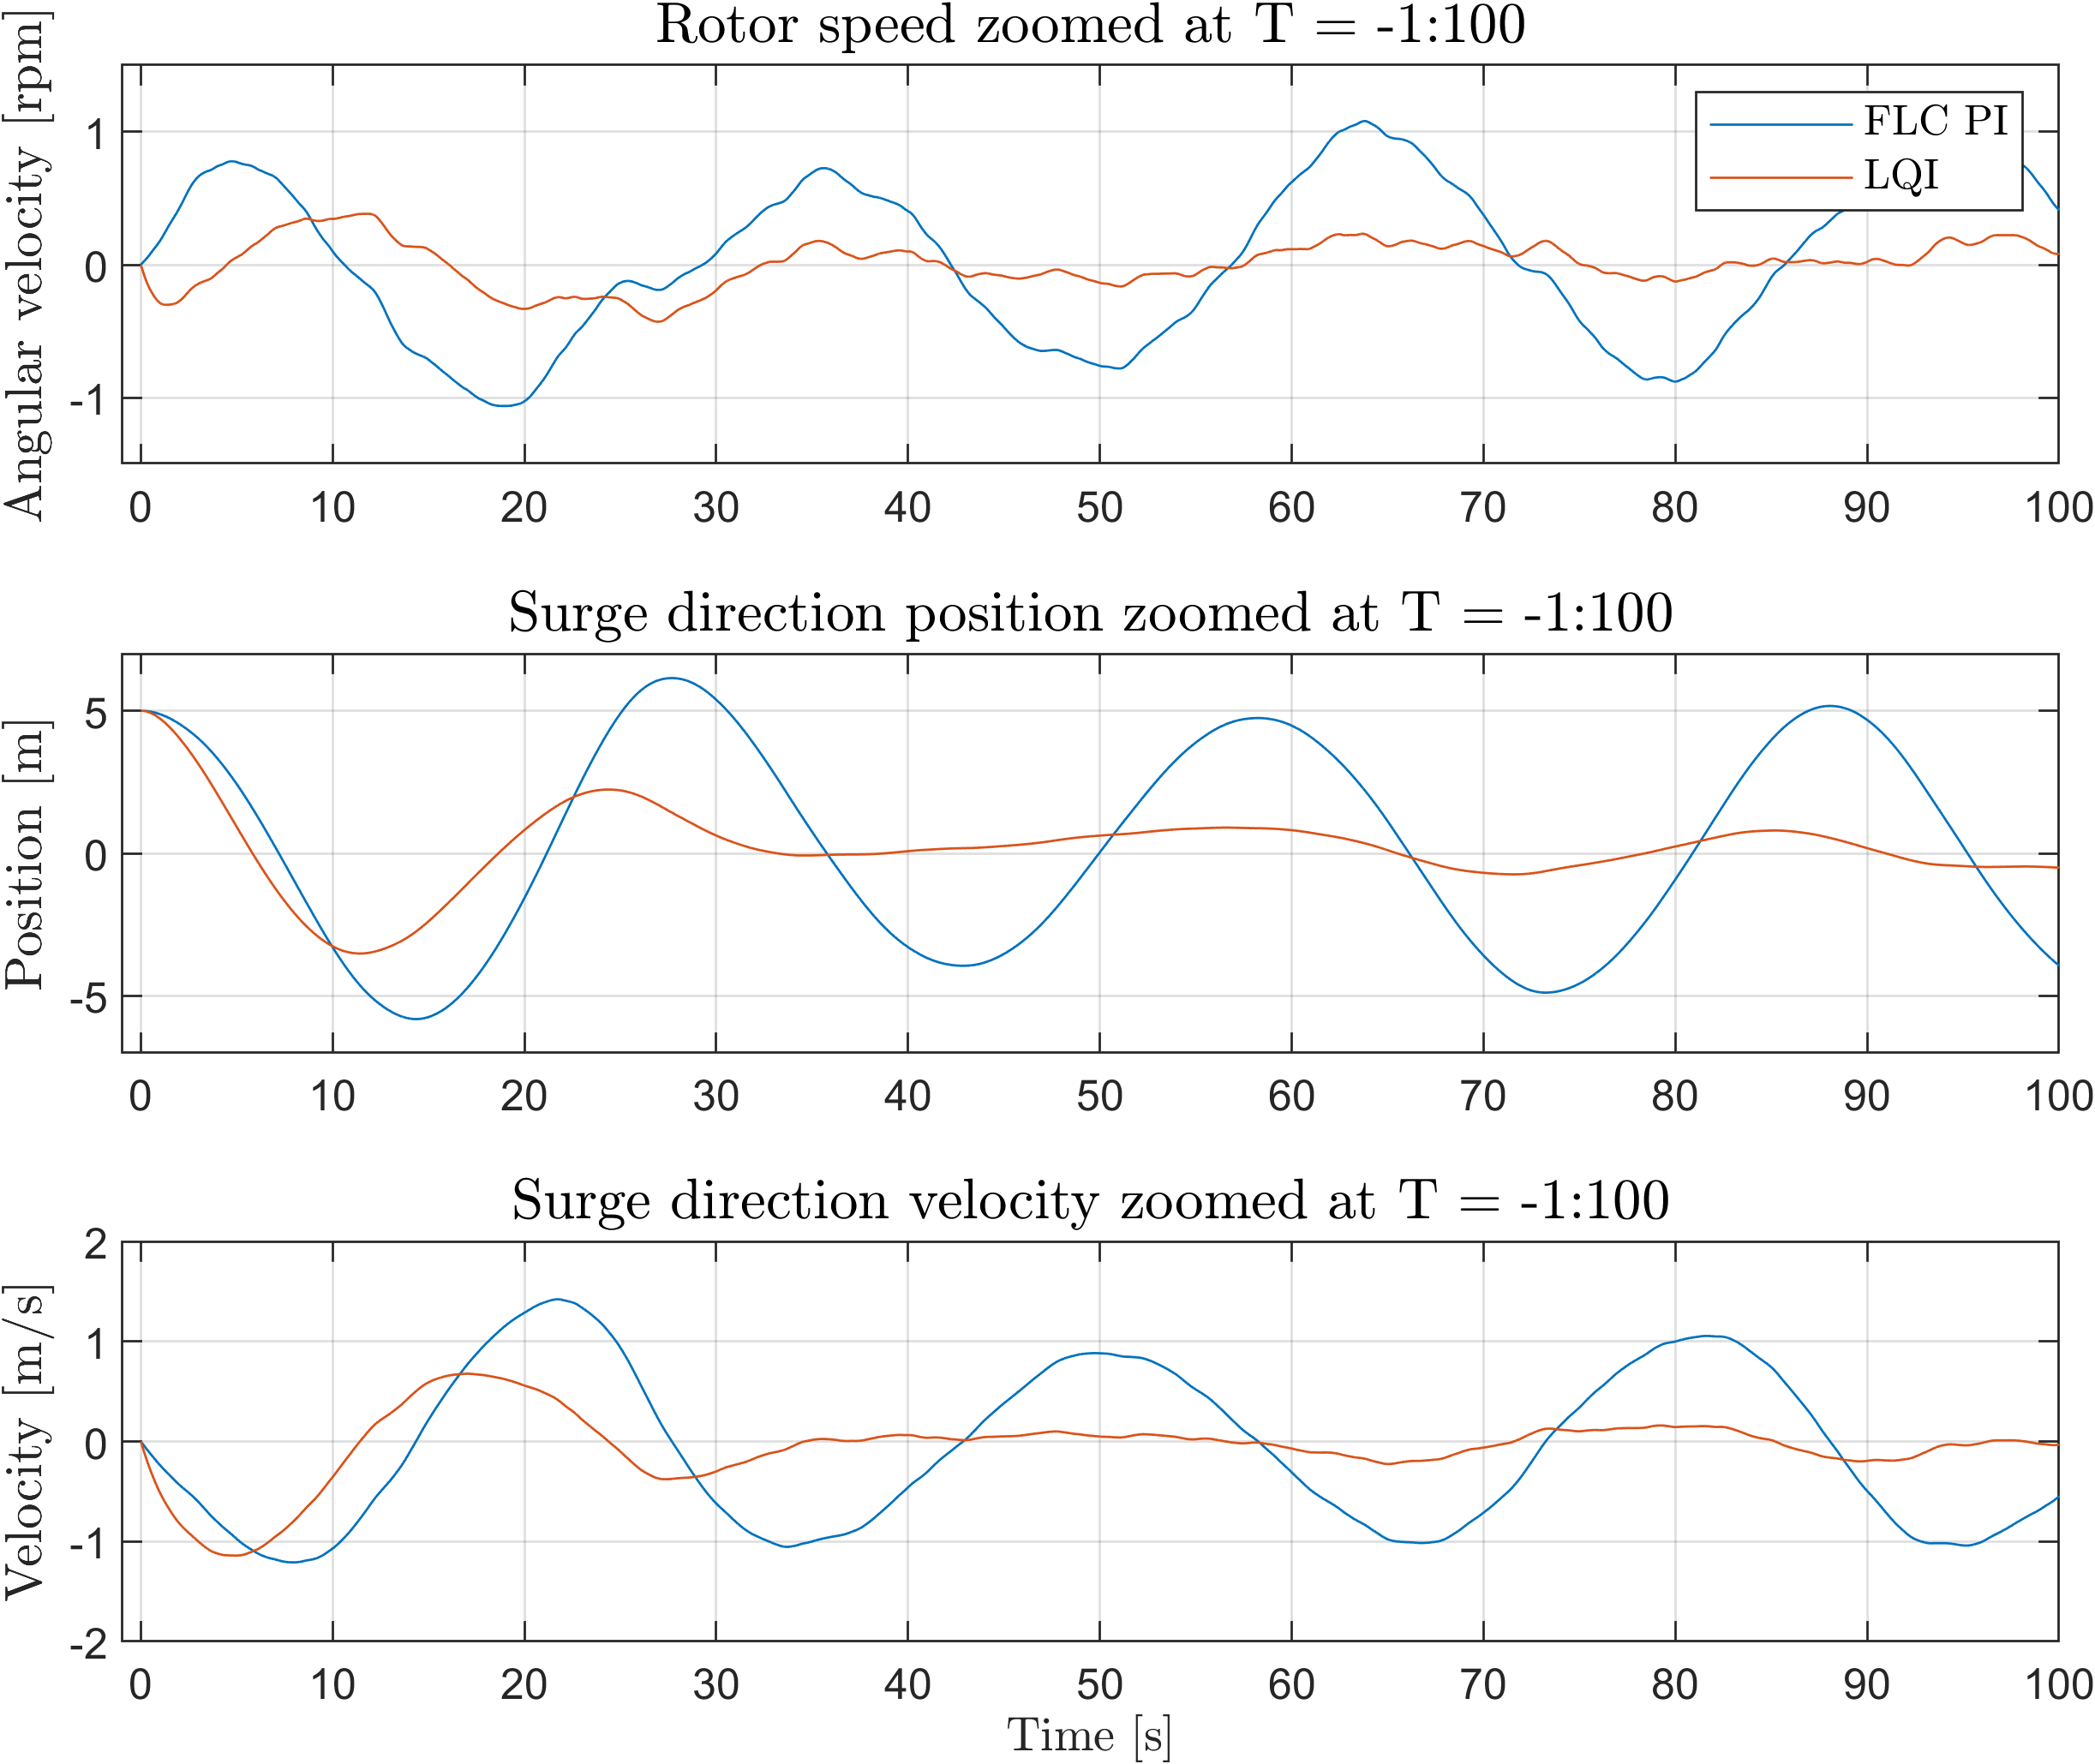
\includegraphics[width=0.7\linewidth]{Graphics/TestResults/linearModPerf/sim_12_W_py_vy_comp_zoom.png}
	\caption{Simulink simulation results. Zoom at the disturbance step.}
	\label{fig:sim_03_W_py_vy_comp_zoom}
\end{figure}

\begin{figure}[ht]
	\centering
	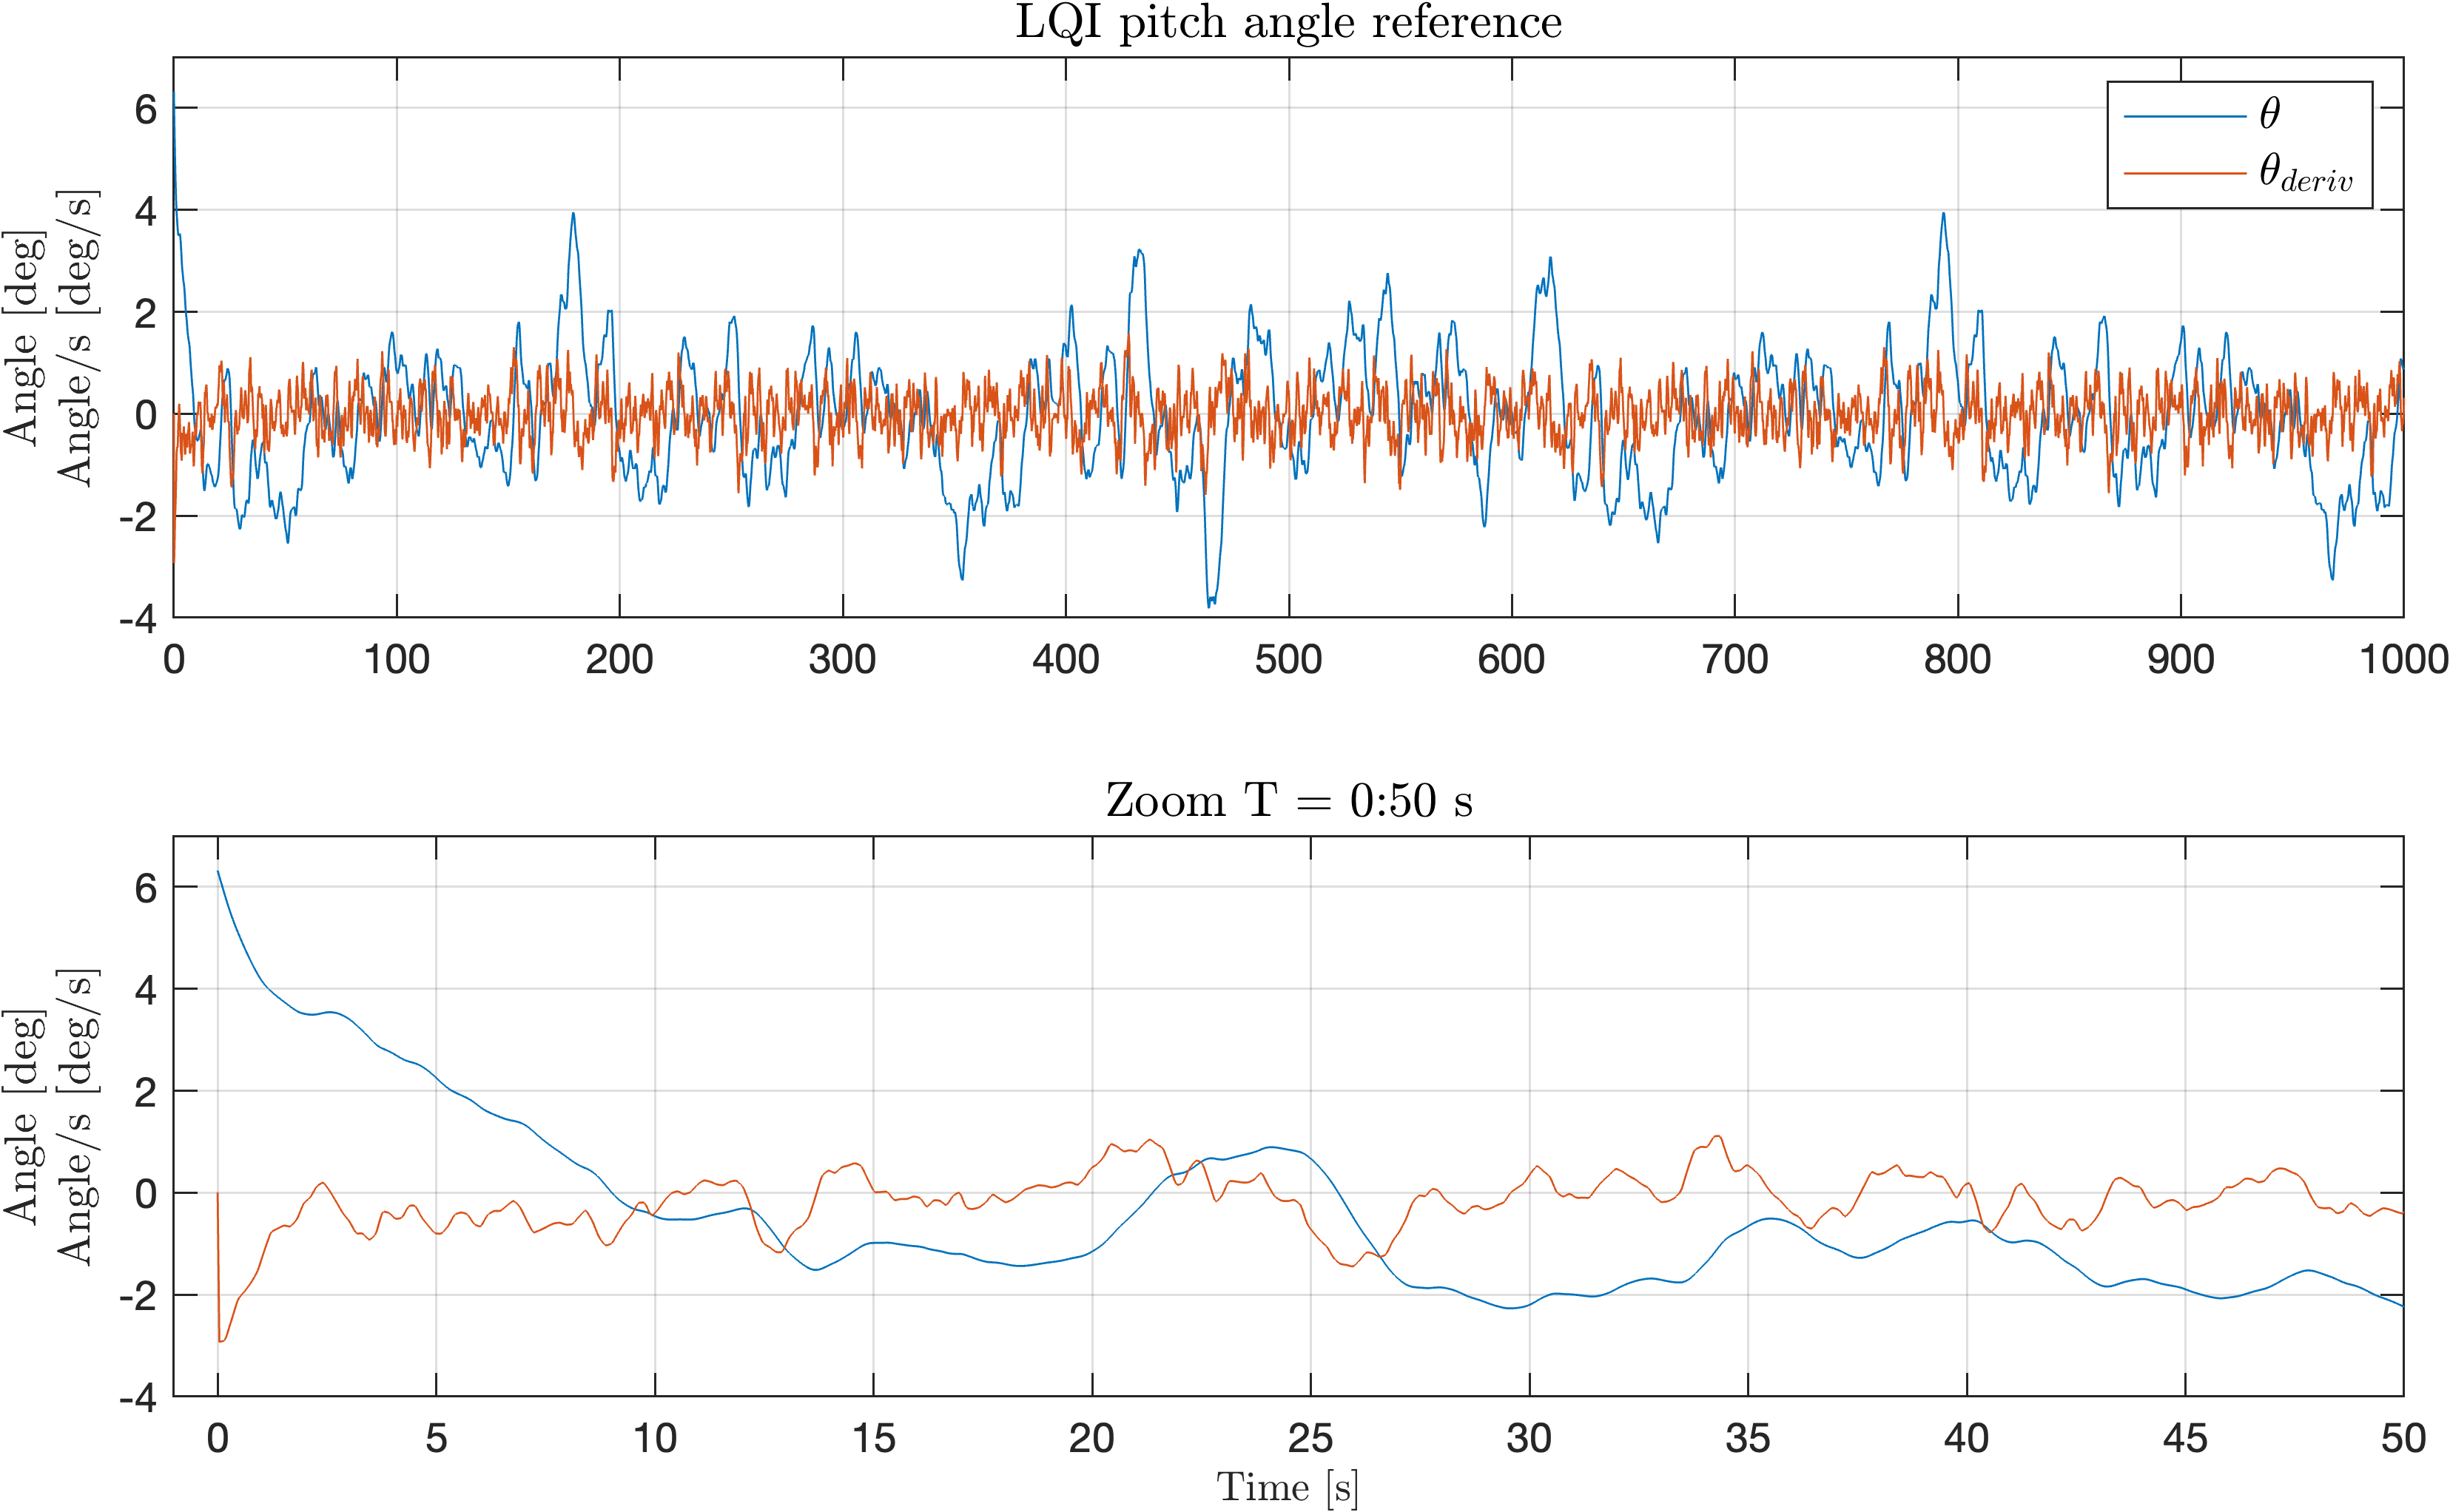
\includegraphics[width=0.7\linewidth]{Graphics/TestResults/linearModPerf/sim_10_pitch.png}
	\caption{Simulink simulation results. Bottom left and right plots are zommed in at 0 to 50 s and 295 to 360 s.}
	\label{fig:sim_01_pitch}
\end{figure}